\documentclass{article}

\usepackage[utf8]{inputenc}
\usepackage{mathtools}
\usepackage{listings}
\usepackage{color}
\usepackage{fancyvrb}
\usepackage{tabularx}
\usepackage{fancyref}
\usepackage{enumitem}
\usepackage{caption}
\usepackage{graphicx}
\usepackage{amsmath}
\usepackage[square,numbers,sort&compress]{natbib}

\title{Molecular Simulation of Materials, Homework 2}
\author{Matthew Grasinger}

\begin{document}

\lstset{language=C++,
        basicstyle=\ttfamily,
        keywordstyle=\color{blue}\ttfamily,
        stringstyle=\color{red}\ttfamily,
        commentstyle=\color{green}\ttfamily,
        morecomment=[l][\color{magenta}]{\#},
        breaklines=true,
        postbreak=\raisebox{0ex}[0ex][0ex]{\ensuremath{\color{red}\hookrightarrow\space}}
}

\pagenumbering{gobble}
\vspace{3.5in}
\maketitle
\clearpage
\pagenumbering{arabic}

\newcommand{\p}{\mathbf{p}}
\newcommand{\pos}{\mathbf{r}}

\section{Problem 1}

\begin{enumerate}[label=\alph*)]
  \item \begin{enumerate}[label=\roman*]
      \item \begin{align*}
          \frac{1}{2m_i} \frac{\partial |\p_i|^2}{\partial \p_i} = & \frac{1}{2m_i} \frac{\partial \left[\p_i \cdot \p_i\right]}{\partial \p_i}, \\
          = & \frac{1}{2m_i} \frac{\partial \left[p_{i1}^2 + p_{i2}^2 + p_{i3}^2\right]}{\partial p_{ij}}, \\
        = & \frac{1}{2m_i} \begin{Bmatrix}2p_{i1} \\ 2p_{i2} \\ 2p_{i3}\end{Bmatrix}, \\
        = & \frac{2 \p_i}{2m_i}, \\
        = & \frac{\p_i}{m_i}.
        \end{align*}
      \item \begin{align*}
          \frac{\partial r_{ij}}{\partial \pos_i} = & \frac{\partial \sqrt{\left(r_{i1} - r_{j1}\right)^2 + \left(r_{i2} - r_{j2}\right)^2 + \left(r_{i3} - r_{j3}\right)^2}}{\partial \pos_i}, \\
        = & \begin{Bmatrix} \frac{1}{2} \left[\left(r_{i1} - r_{j1}\right)^2 + \left(r_{i2} - r_{j2}\right)^2 + \left(r_{i3} - r_{j3}\right)^2\right]^{-1/2} 2\left(r_{i1} - r_{j1}\right) \\ \frac{1}{2} \left[\left(r_{i1} - r_{j1}\right)^2 + \left(r_{i2} - r_{j2}\right)^2 + \left(r_{i3} - r_{j3}\right)^2\right]^{-1/2} 2\left(r_{i2} - r_{j2}\right) \\ \frac{1}{2} \left[\left(r_{i1} - r_{j1}\right)^2 + \left(r_{i2} - r_{j2}\right)^2 + \left(r_{i3} - r_{j3}\right)^2\right]^{-1/2} 2\left(r_{i3} - r_{j3}\right) \end{Bmatrix}, \\
          = & \frac{1}{2} r_{ij}^{-1} 2\pos_{ij}, \\
          = & \frac{\pos_{ij}}{r_{ij}}.
        \end{align*}
      \item
        The Hamiltonian is defined as:
        \begin{align}
          \mathcal{H} = & \mathcal{K} + \mathcal{U}, \\ \label{eq:ham2}
          = & \Sigma_i \frac{\left|\p_i\right|^2}{2 m_i} + \mathcal{U},
        \end{align}
        and the Hamiltonian equations of motion include:
        \begin{align}
          \dot{\pos}_i = & \frac{\partial H}{\partial \p_i}, \\ \label{eq:ham-p}
          \dot{\p}_i = & -\frac{\partial H}{\partial \pos_i}.
        \end{align}
        In order to investigate whether or not the Hamiltonian equations of motion conserve the total system momentum, we want to develop an expression for how the total system momentum is changing with time.
        The total system momentum is given by $\sum_i \p_i$ and consquently its change with time is $\frac{\partial}{\partial t} \left[ \sum_i \p_i \right] = \sum_i \dot{\p}_i$.
        Using \eqref{eq:ham2} and \eqref{eq:ham-p}, we can obtain the expression:
        \begin{align}
          \sum_i \dot{\pos}_i = & -\sum_i \frac{\partial}{\partial \pos_i} \left[ \Sigma_i \frac{\left|\p_i\right|^2}{2 m_i} + \mathcal{U} \right], \\ \label{eq:dpdt}
          = & -\sum_i \frac{\partial \mathcal{U}}{\partial \pos_i}.
        \end{align}
        Recognizing that $-\frac{\partial \mathcal{U}}{\partial \pos_i} = \mathbf{F}_i$, \eqref{eq:dpdt} becomes:
        \begin{align}
          \sum_i \dot{\pos}_i = & \sum_i \mathbf{F}_i, \\ \label{eq:dpdt2}
          = & \sum_i \sum_j \mathbf{F}_i^j,
        \end{align}
        where $\mathbf{F}_i^j$ is the force on particle $i$ due to particle $j$.
        For the interparticle potentials we use in MD, $\mathbf{F}_i^j = -\mathbf{F}_j^i$.
        Thus, the summation on the right-hand side of \eqref{eq:dpdt2} and total system momentum is conserved.

    \end{enumerate}
  \item \begin{align*}
      v_{i,x}(t + \Delta t) & = v_{i,x}(t) + \frac{\partial v_{i,x}}{\partial t}\Bigr|_{t} (\Delta t) + \frac{1}{2} \frac{\partial^2 v_{i,x}}{\partial t^2}\Bigr|_{t} (\Delta t)^2, \\
                            & = v_{i,x}(t) + \frac{F_{i,x}(t)}{m_i} (\Delta t) + \frac{1}{2} \frac{\partial^2 v_{i,x}}{\partial t^2}\Bigr|_{t} (\Delta t)^2.
    \end{align*}
    Recall that $v_{i,x}(t + \Delta t / 2) = v_{i,x}(t) + F_{i,x}(t) \Delta t/(2m_i)$.
    \begin{equation} \label{eq:vi3}
      v_{i,x}(t + \Delta t) = v_{i,x}(t + \Delta t / 2) + \frac{F_{i,x}(t)}{2m_i}(\Delta t) + \frac{1}{2} \frac{\partial^2 v_{i,x}}{\partial t^2}\Bigr|_{t} (\Delta t)^2.
    \end{equation}
    We can simplify \eqref{eq:vi3} further by considering the Taylor expansion of the force:
    \begin{align}
    F_{i,x}(t + \Delta t) & = F_{i,x}(t) + \frac{\partial F_{i,x}}{\partial t}\Bigr|_{t} (\Delta t), \\
                          & = F_{i,x}(t) + \frac{\partial}{\partial t}\left[m_i \frac{\partial v_{i,x}}{\partial t}\right]\Bigr|_{t} (\Delta t), \\
      \label{eq:Ftaylor} & = F_{i,x}(t) + m_i \frac{\partial^2 v_{i,x}}{\partial t^2}\Bigr|_{t}(\Delta t).
    \end{align}
    Dividing both sides of \eqref{eq:Ftaylor} by $2m_i$ and plugging into \eqref{eq:vi3} yields the desired result.
\end{enumerate}

\section{Problem 2}

Given:
\begin{enumerate}[label=\roman*]
  \item $U_s = \frac{x^2}{2}$
  \item $U_s = x^4 - 2x^2 + 1$
\end{enumerate}

The source code for the system with spring potential (i) can be found in \texttt{prob/prob2i.cpp}, and the source code for the systems with spring potential (ii) can be found in \texttt{prob/prob2ii.cpp}.

\begin{enumerate}[label=\alph*)]
  \item Recall: the Hamiltonian is defined as
        \begin{align*}
          \mathcal{H} = & \mathcal{K} + \mathcal{U}, \\ 
          = & \Sigma_i \frac{\left|\p_i\right|^2}{2 m_i} + \mathcal{U},
        \end{align*}
        and the Hamiltonian equations of motion include:
        \begin{align*}
          \dot{\pos}_i = & \frac{\partial H}{\partial \mathbf{r}_i}, \\
          \dot{\p}_i = & -\frac{\partial H}{\partial \pos_i}.
        \end{align*}
        This leads us to
        \begin{align} \label{eq:h1}
          \dot{x} = & \frac{p}{m}, \\ \label{eq:h2}
          \dot{p} = & -\frac{\partial U}{\partial x},
        \end{align}
        for the single mass in the 1-D system.
        For case (i), \eqref{eq:h1} and \eqref{eq:h2} become the following two first order equations
        \begin{align*}
          \dot{x} = & \frac{p}{m}, \\ \label{eq:h2}
          \dot{p} = & -x,
        \end{align*}
        which combined, result in the second order equation
        \begin{equation*}
        m\ddot{x} = -x.
        \end{equation*}

    For case (ii), \eqref{eq:h1} and \eqref{eq:h2} become the following two first order equations
        \begin{align*}
          \dot{x} = & \frac{p}{m}, \\ \label{eq:h2}
          \dot{p} = & -\left(4x^3 - 4x \right),
        \end{align*}
        which combined, result in the second order equation
        \begin{equation*}
        m\ddot{x} = -\left(4x^3 - 4x \right).
        \end{equation*}

   \item \begin{align*}
       m\ddot{x} = & -x, \\
       \ddot{x} + x / m = & 0.
    \end{align*}
    Solving the roots of the characteristic equation $r^2 + 1/m = 0$ results in $r = \pm i \sqrt{1 / m}$ where $i$ is the imaginary number.
    This means the general solution is of the form $x(t) = C_1 \exp \left(i t \sqrt{1 / m} \right) + C_1 \exp \left(-i t \sqrt{1 / m} \right)$.
    Using Euler's formula, we can rewrite this as
    \begin{equation}
      x(t) = A \cos\left(\omega t\right) + B \sin\left(\omega t\right),
    \end{equation}
    where $\omega = \sqrt{1 / m}$.
    We can solve for the constants, $A$ and $B$, using the initial conditions $x(0) = x_0$ and $\dot{x}(0) = v_0$.
    \begin{equation*}
      x(0) = A = x_0.
    \end{equation*}
    And,
    \begin{align*}
      \dot{x}(t) = & -x_0 \omega \sin(\omega t) + B \omega \cos(\omega t), \\
      \dot{x}(0) = & B \omega = v_0. 
    \end{align*}
    Thus, $B = v_0 / \omega$. 
    Recalling that $\omega = \sqrt{1 / m} = 1$, we have the following solutions for the position and velocity of the mass
    \begin{align}
      \label{eq:spos}
      x(t) = & x_0 \cos t + v_0 \sin t, \\ \label{eq:svel}
      \dot{x}(t) = & -x_0 \sin t + v_0 \cos t.
    \end{align}

    To prove that energy is conserved, consider:
    \begin{align*}
      \frac{\partial \mathcal{H}}{\partial t} = & \frac{\partial}{\partial t} \left[ 1/2 \dot{x}^2 + x^2 / 2 \right], \\
      = & \dot{x} \ddot{x} + x \dot{x}. \\
    \end{align*}
    Taking the time derivative of \eqref{eq:svel} results in $\ddot{x} = -x_0 \cos t - v_0 \sin t$.
    Plugging into the above
    \begin{equation*}
      \frac{\partial \mathcal{H}}{\partial t} = \left(-x_0 \sin t + v_0 \cos t\right)\left(-x_0 \cos t - v_0 \sin t\right) + \left(x_0 \cos t + v_0 \sin t\right) \left(-x_0 \sin t + v_0 \cos t\right).
    \end{equation*}
    The right-hand side simplies to zero, thus the change in total energy with time is zero for all of $t$ and energy is conserved. 

    To show momentum is not conserved, consider \eqref{eq:h2}
    \begin{equation*}
      \dot{p} = -\frac{\partial U}{\partial x} = -x.
    \end{equation*}
    The momentum is only not changing when $x = 0$.
    Upon inspection of \eqref{eq:spos}, it is clear that momentum is only conserved for all time in this sytem when $x_0 = v_0 = 0$.
    As this is not the case, momentum is not conserved.
    In a physical sense, momentum is not conserved because, in contrast to the pairwise LJ potential, the sum of the forces, $\sum_i \mathbf{F}_i \neq 0$.

    {\centering
    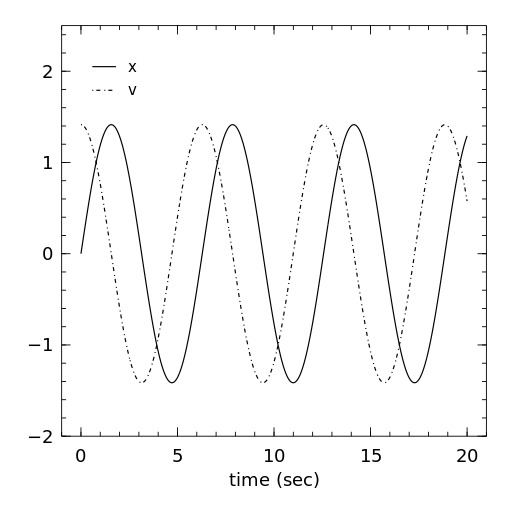
\includegraphics[width=\linewidth]{2b}
    \captionof{figure}{Positions and velocities for $0 \ge t \ge 20$.}
    }

  \item The frequency of the system is given by $\omega = \sqrt{1 / m} = 1$.
    Thus, the time step needed to be much less than $1 \text{ s}$ in order to ensure the vibration of the mass was properly captured.
    I originally chose a time step of $10^{-2} \text{ s}$, however, I found that energy was not being conserved (within a tolerance of $10^{-6}$).
    I reduced the time step to a size of $10^{-4} \text{ s}$ and found that energy \emph{was} indeed being conserved (within a tolerance of $10^{-6}$).

      {\centering
          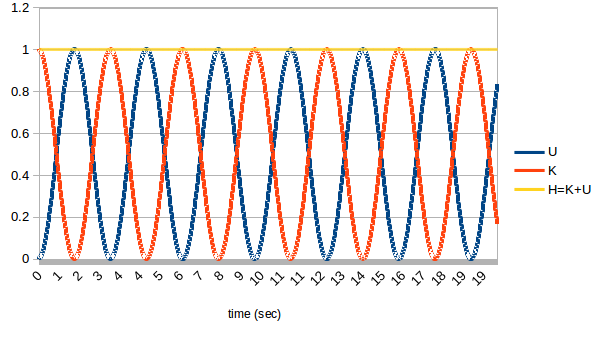
\includegraphics[width=\linewidth]{2c_energy}
          \captionof{figure}{Potential, kinetic, and total energy for $0 \ge t \ge 20$. This shows that energy is conserved.}
      }

    {\centering
    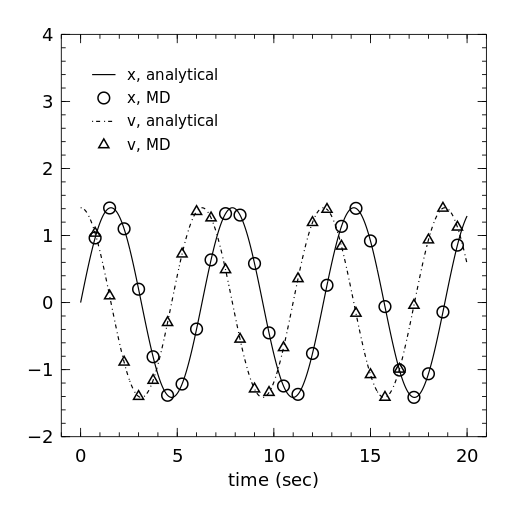
\includegraphics[width=\linewidth]{2c_comparison}
    \captionof{figure}{Positions and velocities for $0 \ge t \ge 20$. Comparison of MD simulation to analytical solution.}
    }

    {\centering
    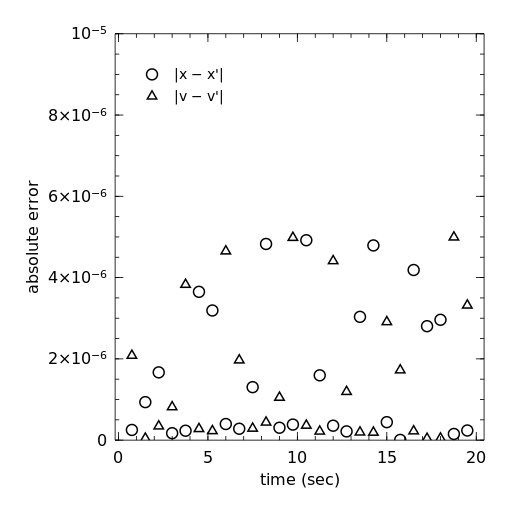
\includegraphics[width=\linewidth]{2c_error}
    \captionof{figure}{Absolute error between MD simulation and analytical solution for both positions and velocities ($0 \ge t \ge 20$).}
    }

    {\centering
    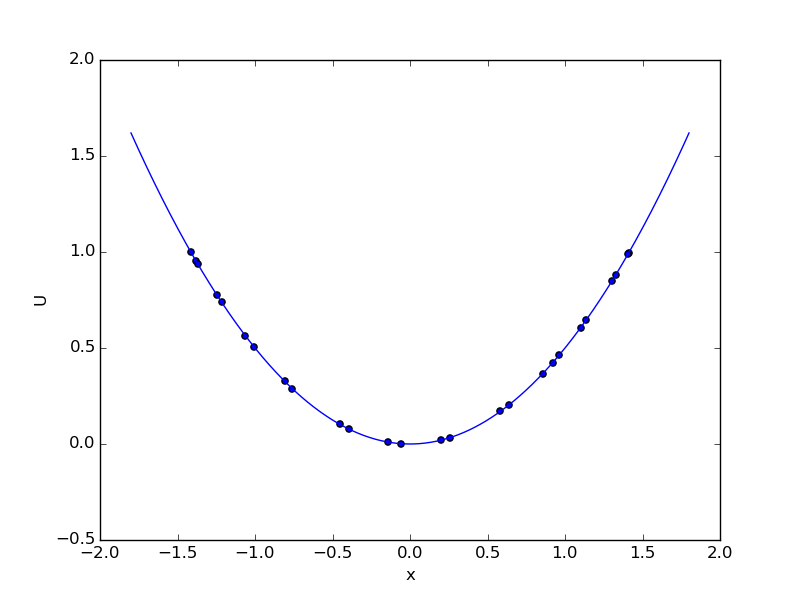
\includegraphics[width=\linewidth]{2c_pot}
    \captionof{figure}{Potential energy with respect to position.}
    }

    {\centering
    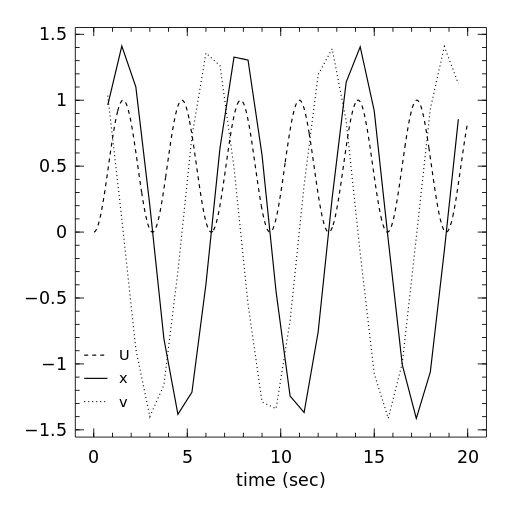
\includegraphics[width=\linewidth]{2c_xvE}
    \captionof{figure}{Potential energy, position, and velocity with time (MD simulation).}
    }

    {\centering
    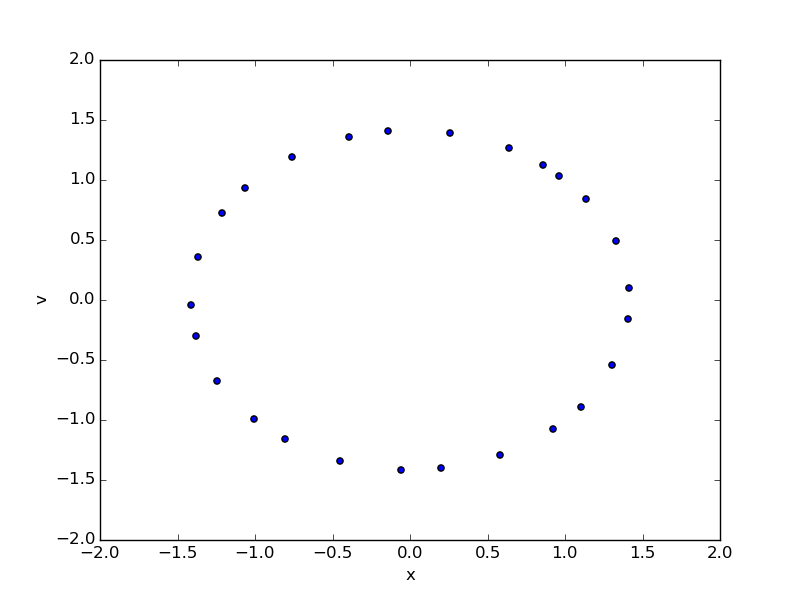
\includegraphics[width=\linewidth]{2c_manifold}
    \captionof{figure}{Constant energy manifold.}
    }

  \item The time step is still valid.

   {\centering
    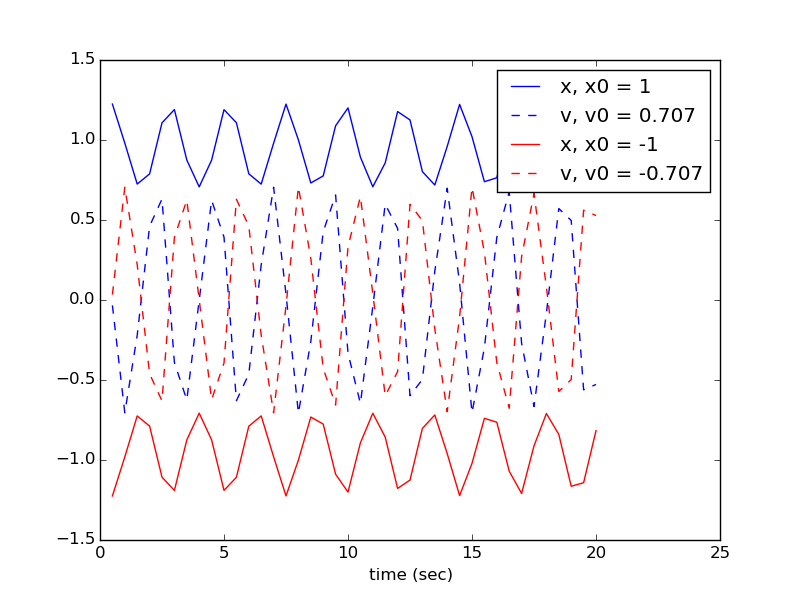
\includegraphics[width=\linewidth]{2d_2ii_025.png}
    \captionof{figure}{Positions and velocities for $0 \ge t \ge 20$. Energy is equal to 0.25.}
    }

   {\centering
    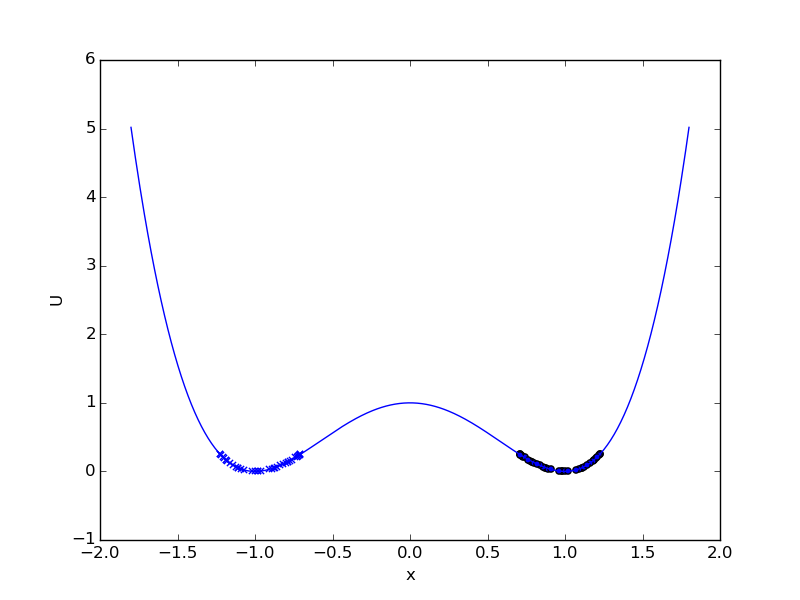
\includegraphics[width=\linewidth]{2d_2ii_025_pot.png}
    \captionof{figure}{Potential energy with respect to position. Energy is equal to 0.25.}
    }

{\centering
    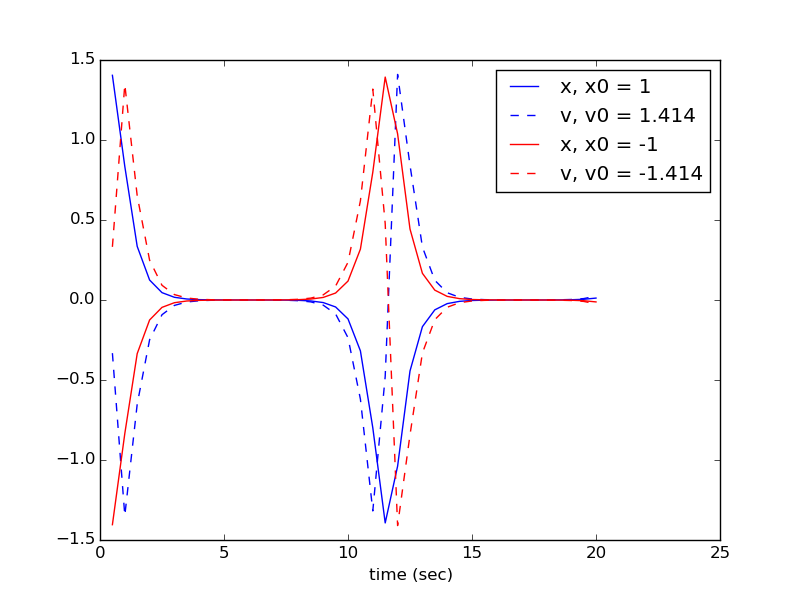
\includegraphics[width=\linewidth]{2d_2ii_100.png}
    \captionof{figure}{Positions and velocities for $0 \ge t \ge 20$. Energy is equal to 1.0.}
    }

   {\centering
    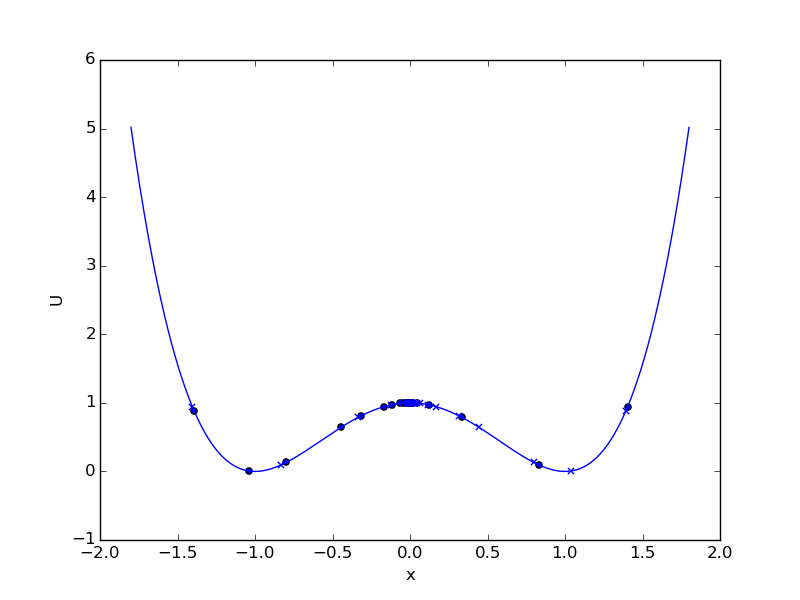
\includegraphics[width=\linewidth]{2d_2ii_100_pot.png}
    \captionof{figure}{Potential energy with respect to position. Energy is equal to 1.0.}
    }

   {\centering
    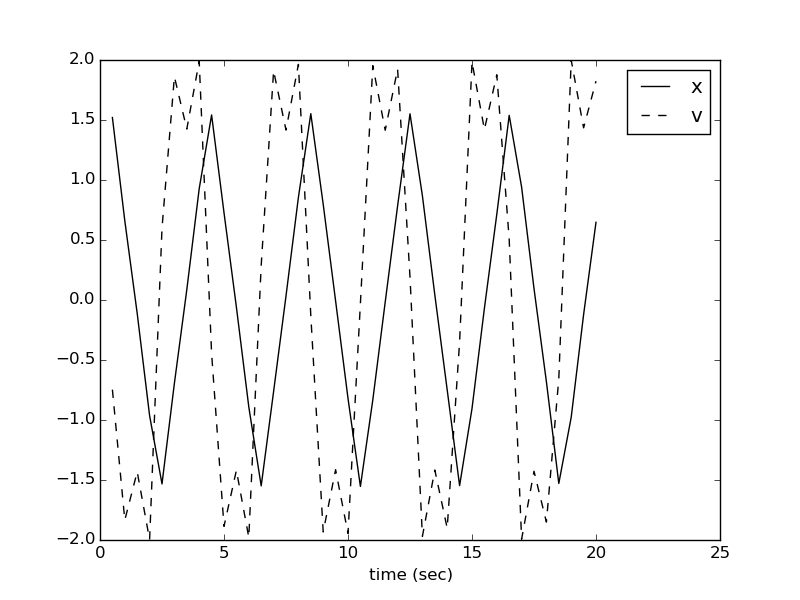
\includegraphics[width=\linewidth]{2d_2ii_200.png}
    \captionof{figure}{Positions and velocities for $0 \ge t \ge 20$. Energy is equal to 2.0.}
    }

   {\centering
    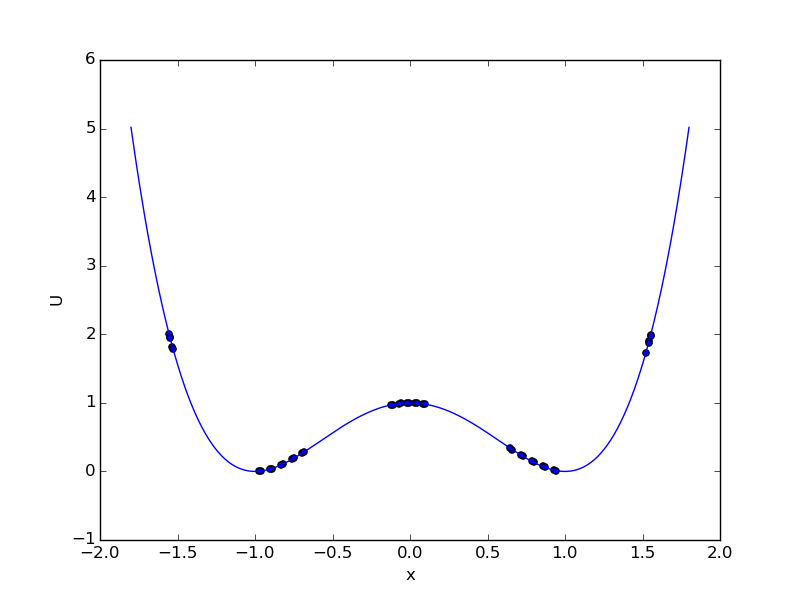
\includegraphics[width=\linewidth]{2d_2ii_200_pot.png}
    \captionof{figure}{Potential energy with respect to position. Energy is equal to 2.0.}
    }

  {\centering
    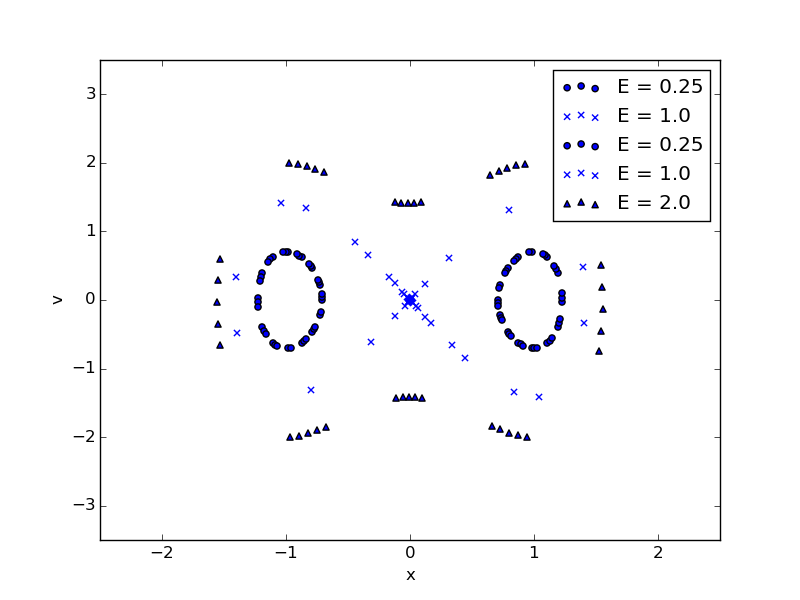
\includegraphics[width=\linewidth]{2d_manifold.png}
    \captionof{figure}{Constant energy manifold for energies 0.25, 1.0, and 2.0}
    }

\end{enumerate}

\section{Problem 3}

The source code can be found in \texttt{prob/prob3.cpp}.

{\centering
    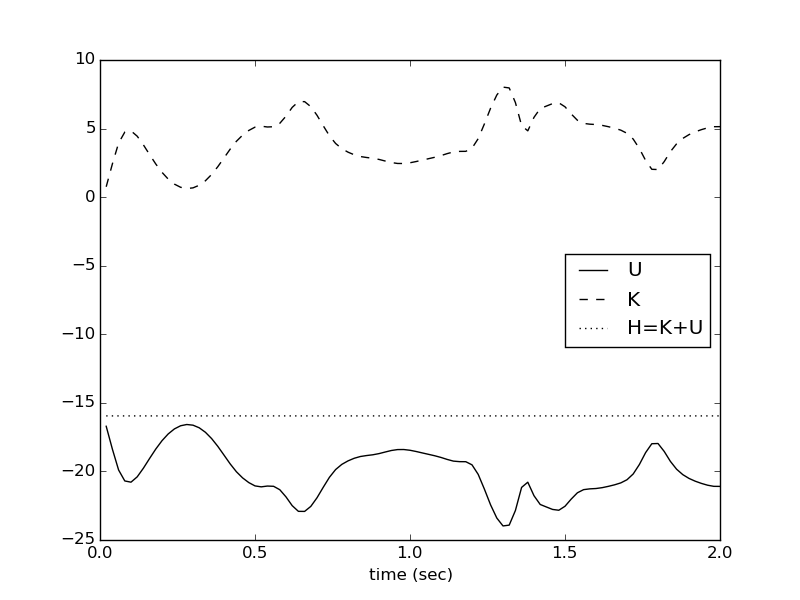
\includegraphics[width=\linewidth]{3_energy.png}
    \captionof{figure}{Potential, kinetic, and total energy for a system of 10 nanoparticles}
    }

{\centering
    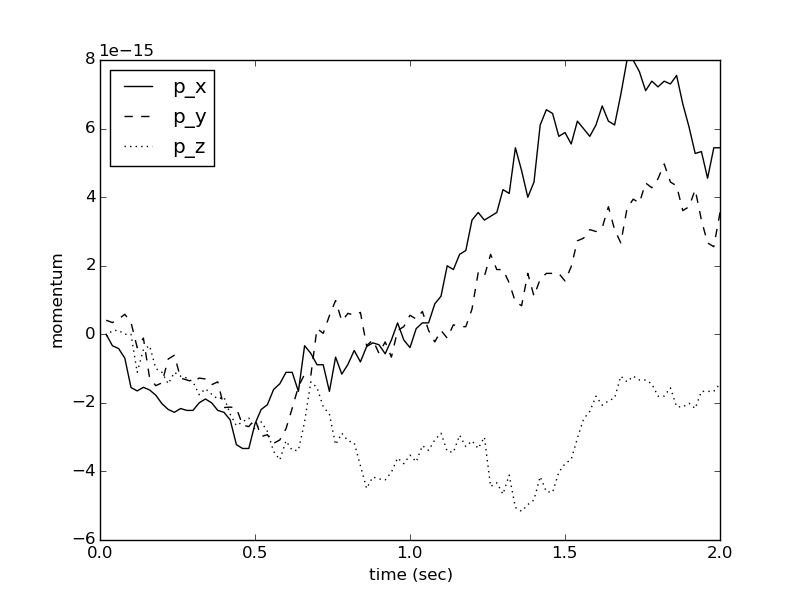
\includegraphics[width=\linewidth]{3_mom.png}
    \captionof{figure}{x, y, and z components of momentum. Momentum is effectively conserved as the largest variation is on the order of $10^{-15}$.}
    }

{\centering
    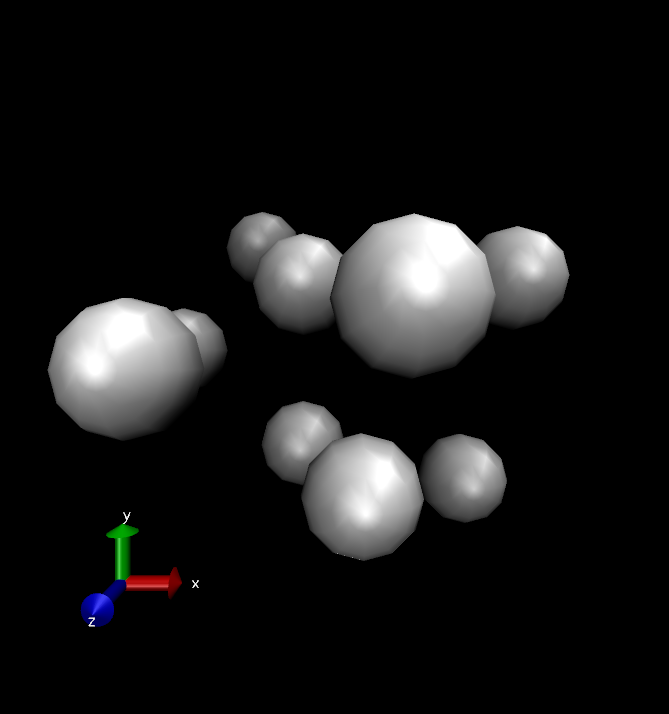
\includegraphics[width=\linewidth]{vmd1}
    \captionof{figure}{Snapshot, $t = 0$.}
    }

{\centering
    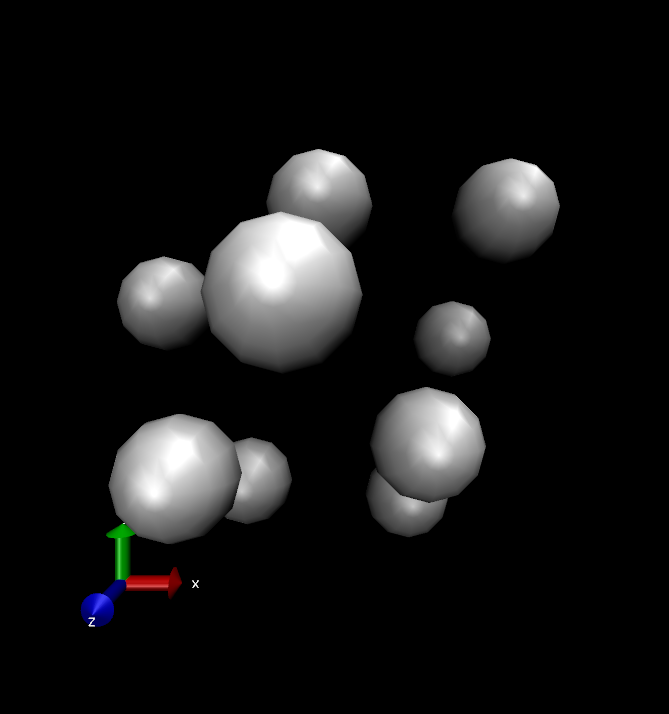
\includegraphics[width=\linewidth]{vmd50}
    \captionof{figure}{Snapshot, $t = 1$.}
    }

{\centering
    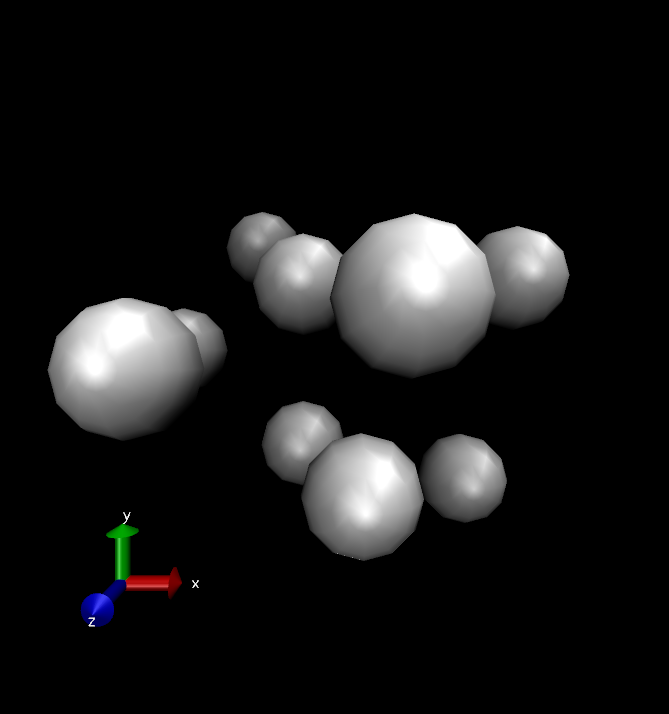
\includegraphics[width=\linewidth]{vmd100}
    \captionof{figure}{Snapshot, $t = 2$.}
    }

\section{Bonus}

The source code can be found in \texttt{prob/bonus.cpp}.
The initial nanoparticle configurations can be found in \texttt{prob/2.txt}, \texttt{prob/3.txt}, \texttt{prob/4.txt}, etc.

The following three figures depict the minimum potential energy plotted against the number of nanoparticles in the simulation ($\eta$ varies from figure to figure).
For the case of $N = 3$, three different initial configuratins were chosen and for $N = 4$ three different initial configurations were chosen.
In each of the three figures, each configuration is plotted as a marker with its $x$ value equal to $N$ and its $y$ value equal to the minimum potential energy.
The scatter of markers for $N = 3$ and $N = 4$ suggests that different minima exist depending not just on the number of particles, but also their initial configuration.

{\centering
    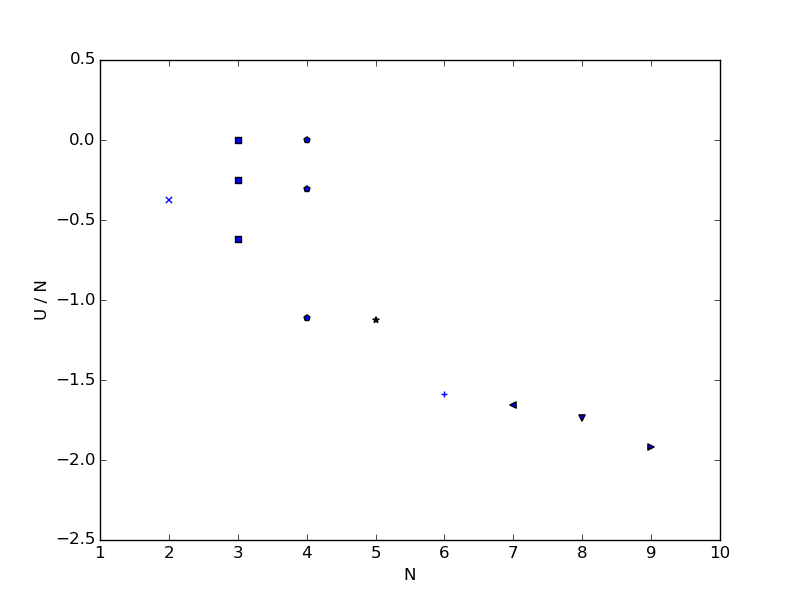
\includegraphics[width=\linewidth]{bonus_eta00001}
    \captionof{figure}{Minimum potential energy (after simulating for $t = 2.0$) with respect to number of nanoparticles, $\eta = 0.0001$.}
    }

{\centering
    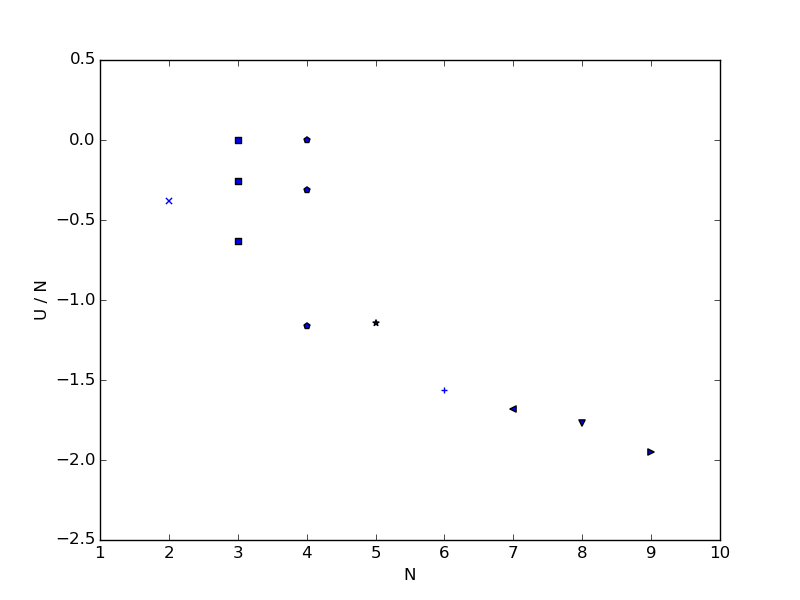
\includegraphics[width=\linewidth]{bonus_eta00100}
    \captionof{figure}{Minimum potential energy (after simulating for $t = 2.0$) with respect to number of nanoparticles, $\eta = 0.01$.}
    }

{\centering
    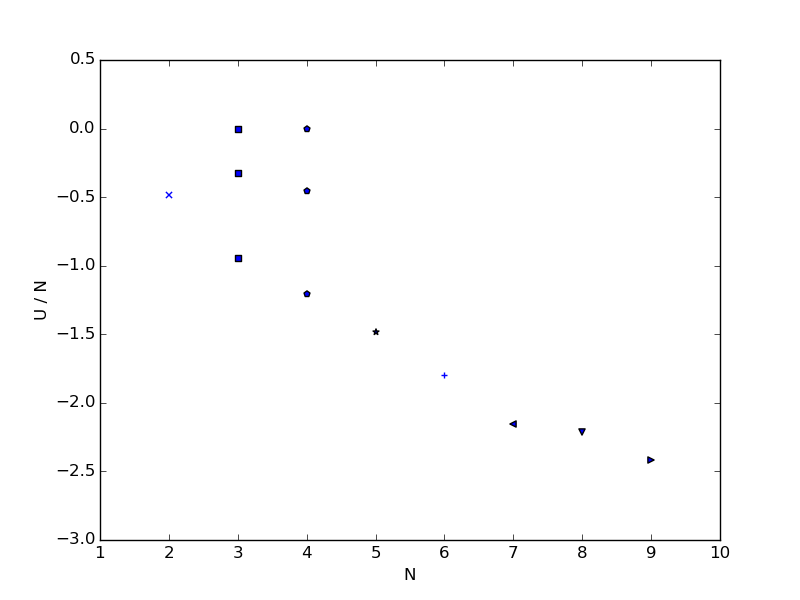
\includegraphics[width=\linewidth]{bonus_eta10000}
    \captionof{figure}{Minimum potential energy (after simulating for $t = 2.0$) with respect to number of nanoparticles, $\eta = 1.0$.}
    }

The last figure clearly shows that the larger the value of the $\eta$ the lower their minimum potential energy per particle for a simulation of the same duration and same number of nanoparticles.
A larger value of $\eta$ also tends to make the $U \ N$ to $N$ relationship appear more linear, i.e. the slope tends to be constant whereas for lower values of $\eta$ the curve tends to level-off at $N \ge 6$.

{\centering
    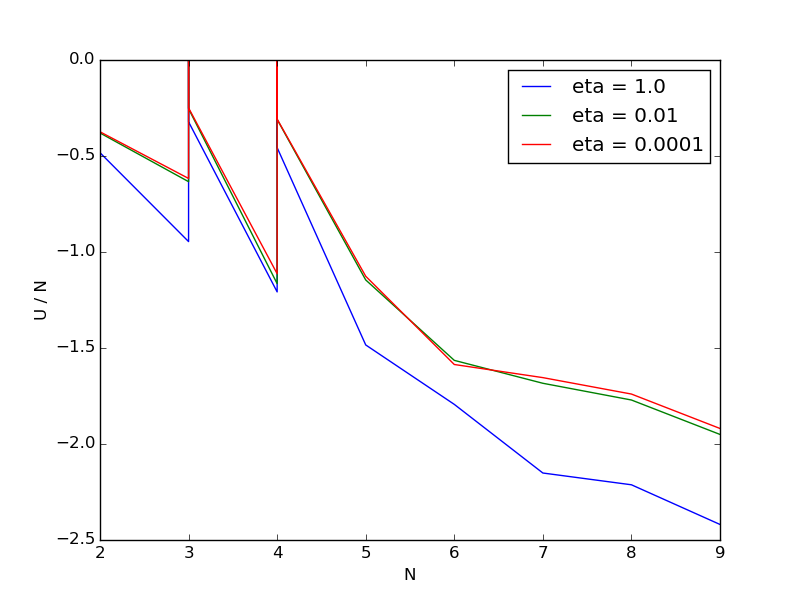
\includegraphics[width=\linewidth]{bonus}
    \captionof{figure}{Minimum potential energy (after simulating for $t = 2.0$) with respect to number of nanoparticles.}
    }

\end{document}
